
\documentclass[
  aspectratio=169, % 16:9 Format
]{beamer}

\usetheme{metropolis} %Berkeley metropolis
\usepackage[utf8]{inputenc}
\usepackage[ngerman]{babel}
\usepackage{graphicx}
\usepackage{amsmath}
\usepackage{booktabs}
\usepackage{siunitx}
\usepackage{hyperref}
\usepackage{float}
\usepackage{xcolor}
\usepackage{pdfpages}
\usepackage{caption} 
\usepackage{media9}
\usepackage[acronym]{glossaries}
\usepackage[T1]{fontenc} 
\usepackage[ngerman]{babel}
\usepackage{capt-of}

% \pdfobjcompresslevel=0
% \pdfcompresslevel=0

% \setbeamercolor{title}{fg=orange}
% \setbeamercolor{frametitle}{fg=orange}
% \setbeamercolor{background canvas}{bg=black!10} % light gray background
\metroset{progressbar=frametitle} % shows progress bar under frame title
% \metroset{progressbar=foot}       % progress bar at footline (default)
% \metroset{progressbar=none}       % hide progress bar
\metroset{sectionpage=none} % disable section pages
% \setbeameroption{show notes}

\definecolor{bar}{rgb}{0, 0.5, 0.2}
\definecolor{frametitle}{rgb}{0.2, 0.2, 0.2}
\setbeamercolor{progress bar}{fg=bar}
\setbeamercolor{background canvas}{bg=white}
\setbeamercolor{frametitle}{fg=white, bg=frametitle}

% Section heading in slides
\setbeamercolor{section title}{fg=blue!80!black}
\makeatletter
\setlength{\metropolis@progressinheadfoot@linewidth}{2pt}  % try 1.5pt or more
\makeatother


\title{Modularbeit Hohlleiterschlitzantenne}
\subtitle{Hochschule München - Antennen und Wellen}
\author{Fynn Gewiese}
\institute{Betreuer: Prof. Dr.-Ing. G. Strauß}
\date{\today}

\setbeamertemplate{footline}{
  \leavevmode%
  \begin{beamercolorbox}[ht=2.5ex,dp=1ex,leftskip=1em,rightskip=1em]{author in head/foot}
    \hfill \insertshorttitle \hfill
    \makebox[0pt][r]{Folie \insertframenumber{} von \inserttotalframenumber\hspace{1em}}
  \end{beamercolorbox}%
}

\begin{document}

\maketitle

\begin{frame}[plain]{\Large \textbf{Inhaltsverzeichnis}}
\begin{columns}[T]
    \begin{column}{0.48\textwidth}
        \begin{minipage}[t]{\linewidth}
            \centering
            \includegraphics[width=\linewidth]{images/bepup.png}
            \captionof{figure}{Drehende Radarantenne\footnotemark}
            \label{fig:marine_radar}
        \end{minipage}
        \footnotetext{\tiny Bildquelle: Wikipedia – \url{https://en.wikipedia.org/wiki/File:Rotating_marine_radar_-_rotating_waveguide_antenna.gif}}
    \end{column}
    
    \begin{column}{0.48\textwidth}
        \vspace{1cm}
        \tableofcontents
    \end{column}
\end{columns}
\end{frame}

\section{Antennentyp}
\begin{frame}{\thesection. Antennentyp}
\begin{columns}[T]

    \begin{column}{0.48\textwidth}
        \centering
        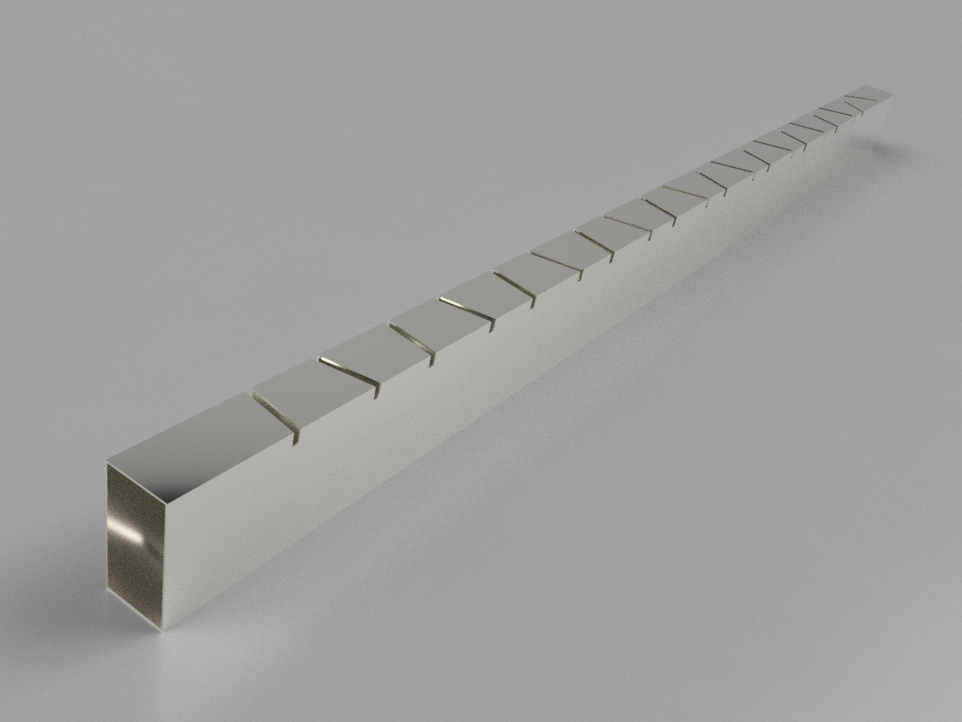
\includegraphics[width=\linewidth]{images/slotted_antenna v1.png}
        \captionof{figure}{3D-Render des Hohlschlitzstrahlers in Fusion360}
        \label{fig:slotted_fusion}
    \end{column}

    \begin{column}{0.48\textwidth}
        \begin{itemize}
            \item Hohlleiterschlitzantenne
            \item Resonanzfall
            \item Kurzgeschlossen an einem Ende
            \item Schlitze in der schmalen Hohlleiterwand
        \end{itemize}
    \end{column}
\end{columns}
\end{frame}

\section{\thesection. Funktionsweise}
\begin{frame}{\thesection. Funktionsweise}
    \begin{figure}
        \centering
        \begin{minipage}[t]{0.49\textwidth}
            \centering
            \includegraphics[width=\linewidth]{images/eplanation.png}
            \caption{Fernfeld bei $\phi = 0^\circ$ (CST Export)}
        \end{minipage}
                \hfill
        \begin{minipage}[t]{0.49\textwidth}
            \centering
            \includegraphics[width=\linewidth]{images/wellenausbreitung.png}
            \caption{Fernfeld bei $\phi = 90^\circ$ (CST Export)}
        \end{minipage}
        \footnotetext{\tiny Quelle: Wikipedia – \url{https://en.wikipedia.org/wiki/File:Rotating_marine_radar_-_rotating_waveguide_antenna.gif}}
    \end{figure}
\end{frame}

\section{\thesection. Richtwirkung}
\begin{frame}{\thesection. Richtwirkung}
    \centering
    \begin{minipage}[t]{\textwidth}
        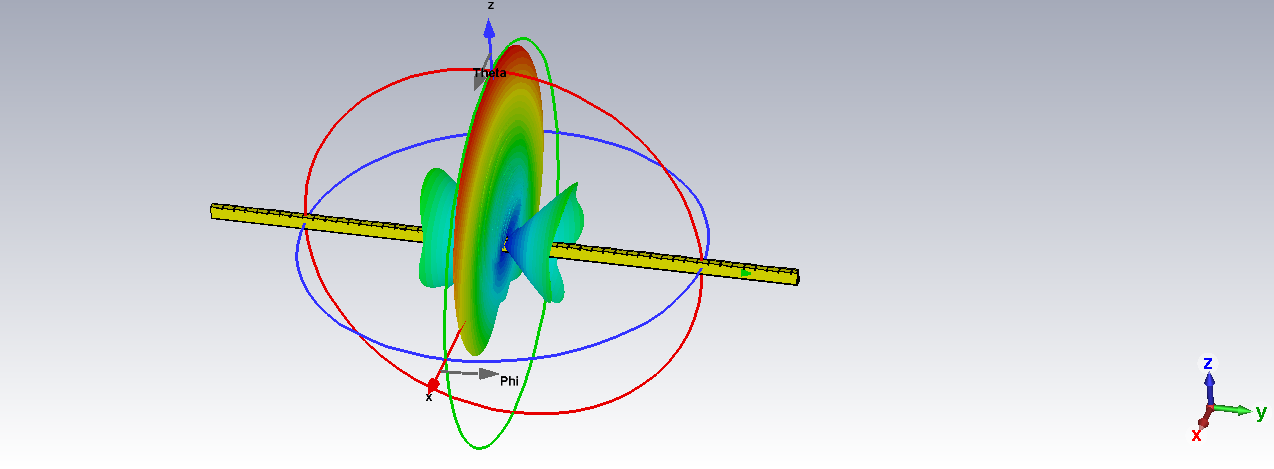
\includegraphics[width=\linewidth]{images/3D_2.png}
        \captionof{figure}{3D-Darstellung der Richtwirkung (CST Render)}
        \label{fig:richtwirkung}
    \end{minipage}
\end{frame}

\section{\thesection. Fernfeld}
\begin{frame}{\thesection. Fernfeld}
    \begin{figure}
        \centering
        \begin{minipage}[t]{0.49\textwidth}
            \centering
            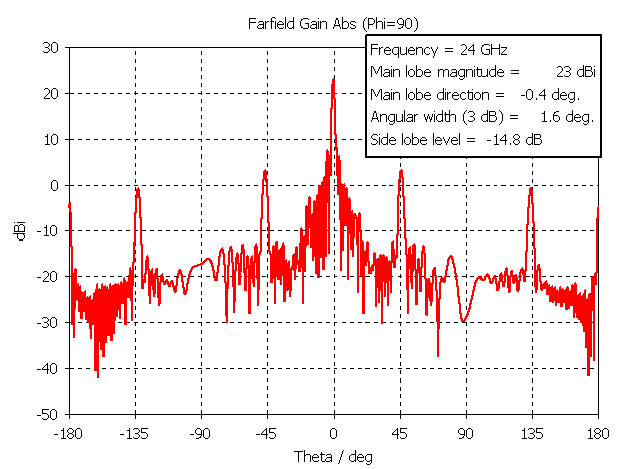
\includegraphics[width=\linewidth]{images/RealGainPh90_Kart.png}
            \caption{Fernfeld bei $\phi = 90^\circ$ (CST Export)}
        \end{minipage}
        \hfill
        \begin{minipage}[t]{0.49\textwidth}
            \centering
            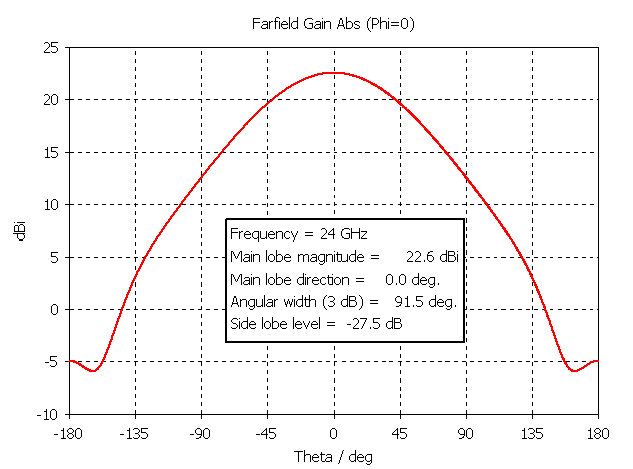
\includegraphics[width=\linewidth]{images/RealGainPh0_Kart.png}
            \caption{Fernfeld bei $\phi = 0^\circ$ (CST Export)}
        \end{minipage}
    \end{figure}
\end{frame}


\section{\thesection. Nahfeld}
\begin{frame}{\thesection. Nahfeld}
    \begin{minipage}[t]{0.48\textwidth}
        \centering
        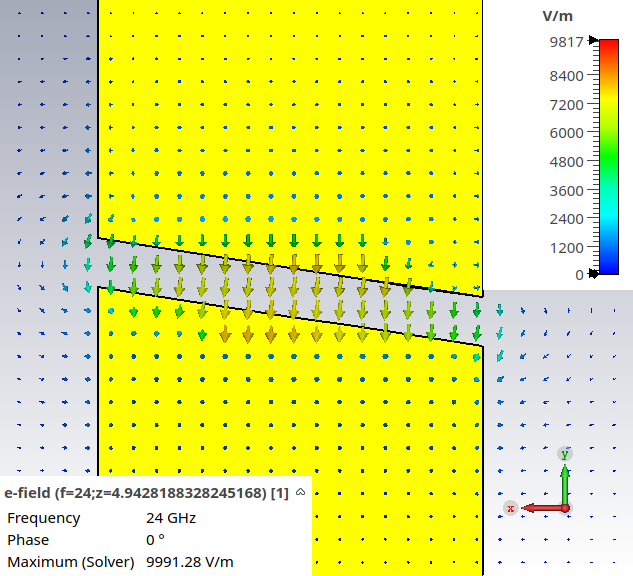
\includegraphics[width=\linewidth]{images/e-field_top_pretty.png}
        \captionof{figure}{Elektrisches Nahfeld (CST Export)}
    \end{minipage}
    \hfill
    \begin{minipage}[t]{0.48\textwidth}
        \centering
        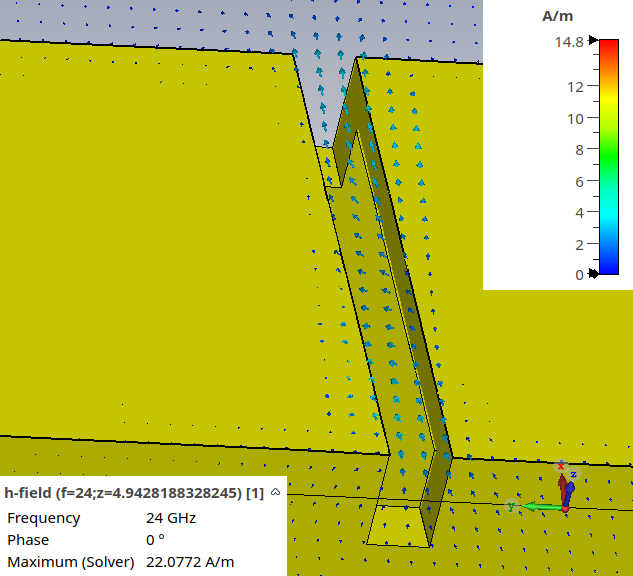
\includegraphics[width=\linewidth]{images/h-field_top_extarct.png}
        \captionof{figure}{Magnetisches Nahfeld (CST Export)}
    \end{minipage}
    \note{
        \begin{minipage}[t]{0.4\textwidth}
            \centering
            \includegraphics[width=\linewidth]{images/eplanation.png}
        \end{minipage}
    }
    \note{\textbf{iplane und hplane cut:}}
\end{frame}

\section{\thesection. Streuparameter|Bandbreite}
\begin{frame}{\thesection. Streuparameter|Bandbreite}
    \begin{minipage}[t]{0.48\textwidth}
        \centering
        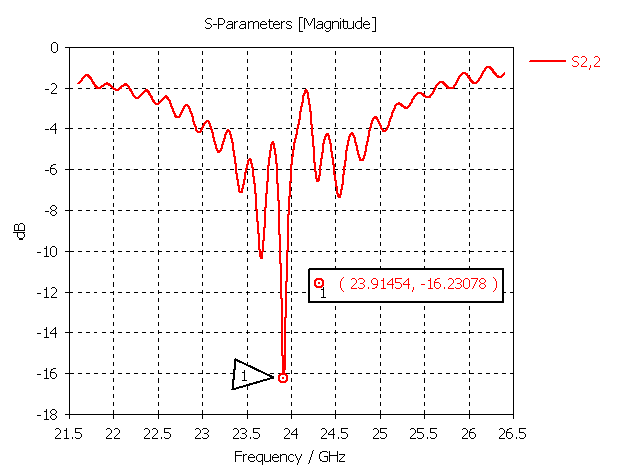
\includegraphics[width=0.9\linewidth]{images/sparamLog.png}
        \captionof{figure}{Reflexionsdämpfung (Logarithmisch)}
    \end{minipage}
    \hfill
    \begin{minipage}[t]{0.48\textwidth}
        \centering
        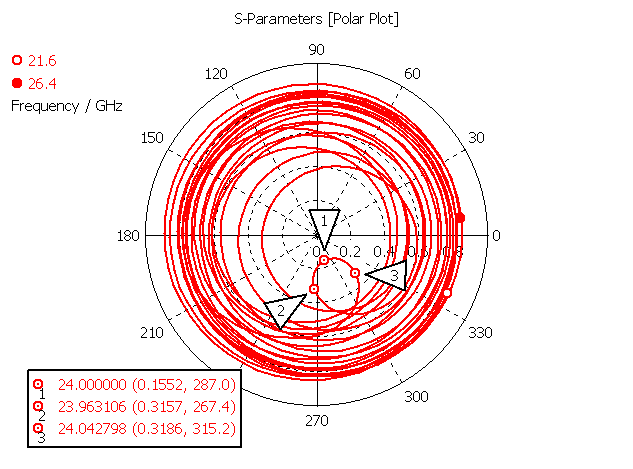
\includegraphics[width=0.9\linewidth]{images/sparamPolar.png}
        \captionof{figure}{Reflexionsdämpfung (Polar)}
    \end{minipage}
\end{frame}


\note{
S₁₁ (Reflexion)
\begin{itemize}
    \item  S₁₁ = 0 dB → 100 Reflexion (schlechtes Matching, z.B. offenes Ende)\\
    \item S₁₁ = –10 dB → ca. 10 reflektierte Leistung, 90 werden übertragen\\
    \item S₁₁ = –20 dB → ca. 1  Reflexion → sehr gutes Matching\\
    \item S₁₁ = –30 dB → ca. 0,1  Reflexion\\
\end{itemize}
}



\section{\thesection. Gewinn}
\begin{frame}{\thesection. Gewinn}
\centering
\begin{itemize}
    \item \textbf{Absoluter Gewinn:} \\
    $G_\text{abs} = 23{,}4\,\mathrm{dBi}$ 
    
    \note{\textbf{Absoluter Gewinn:} Strahlungsverstärkung der Antenne inklusive interner Verluste (z.\,B. Leitungsverluste, Dielektrika), aber ohne Berücksichtigung des Rückflussverlusts (\gls*{s11}).\\}
    
\item \textbf{Realisierter Gewinn:}
\begin{flushleft}
G_\text{real} &= G \cdot (1 - |S_{11}|) \\
&= 23{,}4\,\mathrm{dBi} \cdot (1 - 0{,}158489) \\
&\approx 19{,}7\,\mathrm{dBi}
\end{flushleft}

    \note{\textbf{Realisierter Gewinn:} Das, was nach allen Verlusten und Rückkopplungen (\gls*{s11}) noch abgestrahlt wird – also der realistischste Wert.\\}
    
    % \item Richtwirkung: °
    % \note{\textbf{Richtwirkung:} Maß dafür, wie stark die Antenne in eine Richtung abstrahlt verglichen mit einer isotropen Antenne – ohne Verluste durch R\"uckkopplung oder ohmsche Verluste.\\}
    
    % \item \gls*{hpbw}: °
    % \note{\textbf{\gls*{hpbw} (Half Power Beam Width):} Der Winkelbereich, in dem der Antennengewinn nicht mehr als 3\gls*{db} unter dem Maximalwert liegt. Gibt an, wie breit der Hauptstrahl ist.\\}
    
    % \item \textbf{Plausibilität:} \\
    % ($G_\text{real} = Direct - |\gls*{s11}|$)
    % \note{\textbf{Plausibilität:} Überprüfen, ob Realized Gain = Directivity \– Rückflussverlust (aus z.\,B. \gls*{s11}). Typisch: \gls*{s11} bei \−10\gls*{db} entspricht ca. 0.5\gls*{db} Verlust.\\}
\end{itemize}
\end{frame}

\begin{frame}{\thesection. Berechnungen}
\footnotesize
\begin{tabular}{@{}p{0.15\textwidth}p{0.35\textwidth}p{0.45\textwidth}@{}}
\textbf{Größe} & \textbf{Allgemein} & \textbf{Für meine Schlitzantenne} \\
\midrule
HPBW & $\text{HPBW}_\text{uni} \approx \dfrac{50{,}76^\circ}{N \cdot d/\lambda}$ 
& $N = 50$, $d = 8{,}74$ mm, $\lambda = 12{,}45$ mm \newline
$\Rightarrow \text{HPBW} \approx \mathbf{1{,}4^\circ}$ \\
\midrule
Richtwirkung Dipol & $D_\text{hertz} = \dfrac{3}{2} \approx 1{,}76$ dBi 
& Nicht relevant für Gruppenstrahler \\
\midrule
HPBW Dipol & $\text{HPBW}_\text{hertz} = 90^\circ$ 
& Gilt vertikal für jeden Schlitz (dipolähnlich) \\
\midrule
Richtwirkung Gesamt & $\displaystyle D \approx \dfrac{41253}{\Theta_\text{min} \cdot \Theta_\text{max}}$ 
& Mit $\Theta_\text{min} \approx 1{,}4^\circ$, $\Theta_\text{max} \approx 90^\circ$ \newline
$\Rightarrow D \approx \mathbf{327}$ \\
\end{tabular}

\vspace{3mm}
\footnotesize
\textbf{Parameter:} \\
$N$: Anzahl der Strahlerelemente, \quad
$d$: Abstand zwischen den Elementen, \quad
$\lambda$: Wellenlänge, \\
$\text{HPBW}$: Halbwertsbreite der Hauptkeule (3 dB), \quad
$D$: Richtwirkung (Direktivität), \quad
$\Theta_\text{min}, \Theta_\text{max}$: kleinste bzw. größte 3-dB-Keulenbreite (in Grad)
\end{frame}

\section{\thesection. Spezifikationen: Ziel vs. Umsetzung}

\begin{frame}{\thesection. Spezifikationen: Mechanisch}
\begin{columns}[T]
  \begin{column}{0.4\textwidth}
    \begin{minipage}[t]{\linewidth}
         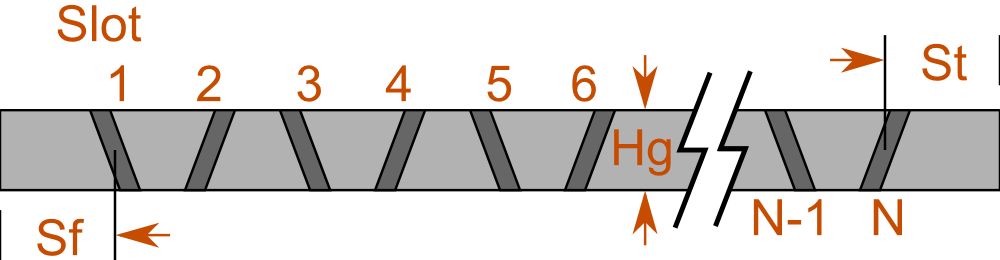
\includegraphics[width=\linewidth]{images/sideviewscets.png}
        \captionof{figure}{Skizze des Hohlleiters aus Antenna Magus}
        \label{fig:magus_sketch}
    \end{minipage}
  \end{column}

  \begin{column}{0.7\textwidth}
    \centering
    \scriptsize
    \textbf{Mechanische Parameter}
    \vspace{1mm}

    \begin{tabular}{|l|c|c|c|}
      \hline
      \textbf{Parameter} & \textbf{Gewünscht} & \textbf{Berechnet} & \textbf{Simuliert} \\
      \hline
      Anzahl Slots & – & – & \textbf{50} \\
      \hline
      Slotabstand & – & – & 8{,}74~mm \\
      \hline
      Slotbreite & – & $\lambda/20$ & 624{,}6~µm \\
      \hline
      Antennenlänge & – & – & 14{,}4~cm \\
      \hline
      Material & Silber & – & Silber \\
      \hline
    \end{tabular}

    \vspace{2mm}
    \scriptsize Realisierung durch Einschränkungen von Antenna Magus limitiert
  \end{column}
\end{columns}

\note{\textbf{Slotbreite:}
$\lambda$/20: Schmal genug, um als einfacher Schlitzstrahler zu funktionieren (kein Multimodenverhalten), aber breit genug, um Leistung zu koppeln und mechanisch herstellbar zu sein.\\
Breiter als $\lambda$/10: Mehrere Moden möglich (unerwünscht), mehr Rückreflexion (Impedanzproblem), ungenaue Strahlungsrichtung.\\
Schmaler als $\lambda$/30: Kopplung verschlechtert sich, geringerer Wirkungsgrad, Fertigung wird kritisch.\\}
\end{frame}

\note{
\newpage
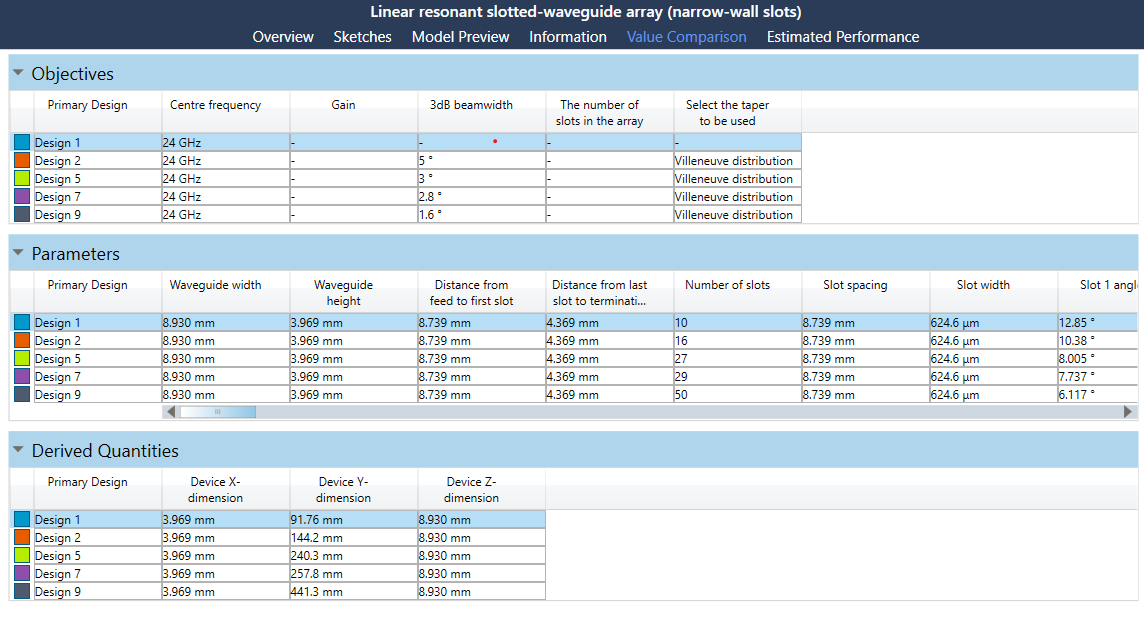
\includegraphics[width=\linewidth]{images/slotNCompariosn.png}
\newpage
\includegraphics[width=0.5\linewidth]{images/reflection_diag.png}
}

\begin{frame}{\thesection. Spezifikationen: Elektrisch}
\begin{columns}[T]
  
  \begin{column}{0.7\textwidth}
    \centering
    \scriptsize
    \textbf{Elektrische Parameter}
    \vspace{1mm}

    \begin{tabular}{|l|c|c|c|}
      \hline
      \textbf{Parameter} & \textbf{Gewünscht} & \textbf{Berechnet} & \textbf{Simuliert} \\
      \hline
      Frequenz (Mittenfrequenz) & 24.0~\gls*{ghz} & – & 24.0~GHz \\
\hline
Maximaler Gewinn & – & – & 23{,}0~dBi (hor) \textbar{} 22{,}6~dBi (vert) \\
\hline
Realisierter Gewinn & – & – & 22{,}8~dBi (hor) \textbar{} 22{,}4~dBi (vert) \\
\hline

      % Maximaler Gain (vertikal) & – & – & 22.6~dBi \\
      % \hline
      % Realisierter Gain (vertikal) & – & – & 22.4~dBi \\
      % \hline
      Horizontale 3~dB-Keulenbreite & \texttt{<=} 1.0° & 1.4° & \textcolor{red}{1.6°} \\
      \hline
      Vertikale 3~dB-Keulenbreite & – & 90° (Dipol) & 91.5° \\
      \hline
      Richtwirkung & – & 327 & 219 \\
      \hline
    \end{tabular}
  \end{column}
\end{columns}

\note{\textbf{Wellenlänge:} $\lambda$=C/f, hier: 12.49 mm\\
\textbf{Slotabstände:} Gewählt damit die Antenne in Phase abstrahlt\\
\textbf{Anzahl an Slots:} Mehr Slots: Geringere Bandbreite, höherer Gewinn.\\
\textbf{Antennenlänge:} Hat nichts mit Frequenz zu tun, einfach länger mit mehr Slots\\
\textbf{E-Plane:} Quer zur Schlitzrichtung \\
\textbf{H-Plane:} Entlang der Schlitzrichtung\\
}
\end{frame}

\section*{\thesection. Abkürzungen}
\begin{frame}{\thesection. Abkürzungen}
\scriptsize
\begin{tabular}{|l|l|}
\hline
\textbf{Abkürzung} & \textbf{Bedeutung} \\
\hline
HPBW        & Half Power Beam Width (Halbwertsbreite) \\
HPBWhor     & Horizontal Half Power Beam Width (horizontale Halbwertsbreite) \\
dBi         & Dezibel gegenüber Isotropstrahler \\
dB          & Dezibel \\
S11         & Rückflussdämpfung (Reflexionsfaktor) \\
GHz         & Gigahertz \\
mm          & Millimeter \\
µm          & Mikrometer \\
$\lambda$   & Wellenlänge (Wavelength) \\
$f$         & Frequenz \\
E-Feld      & Elektrisches Feld \\
H-Feld      & Magnetisches Feld \\
CST         & Computer Simulation Technology \\
\hline
\end{tabular}
\end{frame}

\section*{\thesection. Literatur}
\begin{frame}[allowframebreaks]{\thesection. Literatur}
\begin{thebibliography}{}

\bibitem{strauss}
G. Strauß: \textit{Antennen und Wellen}.\\ Manuskript, Pasing: Hochschule Muenchen, Maerz 2022

\bibitem{compactslot}
Kumar, K. P. Ray: \textit{Compact Slot Array Antennas for Wireless Communications},\\ Academic Press, 2019

\bibitem{Fusion}
Autodesk Fusion 360, Autodesk Inc., www.autodesk.com/products/fusion-360

\bibitem{CST}
CST Studio Suite, Version 2023, Dassault Systèmes, www.3ds.com/products-services/simulia/products/cst-studio-suite

\bibitem{Maggus}
Antenna Magus, Version 2023.2, Dassault Systèmes, www.antennamagus.com

\end{thebibliography}
\end{frame}

% \section*{Abbildungsverzeichnis}
% \begin{frame}{Abbildungsverzeichnis}
% \listoffigures
% \end{frame}

\includepdf[pages=-]{Aufgaben_AundW_SS2025_.pdf}
\includepdf[pages=-]{hinweise_zur_praesention_modularbeiten(1).pdf}

\end{document}
